% This is samplepaper.tex, a sample chapter demonstrating the
% LLNCS macro package for Springer Computer Science proceedings;
% Version 2.20 of 2017/10/04
%
\documentclass[runningheads]{llncs}
%\documentclass{article}
%
\usepackage{graphicx}
% Used for displaying a sample figure. If possible, figure files should
% be included in EPS format.
%
% If you use the hyperref package, please uncomment the following line
% to display URLs in blue roman font according to Springer's eBook style:
% \renewcommand\UrlFont{\color{blue}\rmfamily}

\begin{document}
%
\title{Network Intrusion Detection and Prevention\thanks{Supported by FH Aachen University of Applied Sciences.}}
%
%\titlerunning{Abbreviated paper title}
% If the paper title is too long for the running head, you can set
% an abbreviated paper title here
%
%\author{Ali Coban\inst{1}\orcidID{0000-1111-2222-3333} \and
%Jasmin Bauer\inst{2,3}\orcidID{1111-2222-3333-4444} \and
%Nils Nitsch\inst{3}\orcidID{2222--3333-4444-5555}}
%
%\authorrunning{F. Author et al.}
% First names are abbreviated in the running head.
% If there are more than two authors, 'et al.' is used.
%
\institute{Fachhochschule Aache, Eupenerstraße 70, 52066 Aachen, Germany \and
Springer Heidelberg, Tiergartenstr. 17, 69121 Heidelberg, Germany
\email{lncs@springer.com}\\
\url{https://www.fh-aachen.de/}\\
\url{http://www.springer.com/gp/computer-science/lncs}}
%
\maketitle              % typeset the header of the contribution
%
\begin{abstract}
Seit den frühen Anfängen des Internets, sogenannte "Internet Epidemien" haben weltweit enormen Schaden verursacht und gefährden die Sicherheit der Systeme bis heute noch.
Als Internet Epidemien bezeichnet man bösartige Software die sich selbständig über das Internet verteilen kann. Als Beispiel gab es 1988 den sogenannten "Morris worm". Dieser schaffte es, 10\% aller Internet Hosts zu infizieren. Im Jahre 2001 schaffte es der "Code Red Worm" mehr als 350.000 Internet Hosts innerhalb eines Tages zu kompromittieren.
Network Intrusion Detection ist ein neuartiges Vorgehen, um in bestehenden Computern oder Netzwerken eine Art Sicherheit darzustellen, während diese weiterhin in ihrem "offenen" Modus operieren können.
Das Ziel der Intrusion Detection ist es, wenn möglich in Echtzeit, unautorisierte Zugriffe oder ein Misshandeln des Systems zu identifizieren. 

Ein Grund, warum Intrusion Detection heutzutage eine schwierige Aufgabe darstellt, ist die Vermehrung heterogener Netwerke durch die vermehrte Konnektivität von Computersystemen. Dadruch wird es Angreifern einfacher gemacht, auf diese Systeme zuzugreifen.

Intrusion Detection Systems (IDS) basieren auf der Vermutung, dass unautorisierte Zugriffe erkennbar sind, als auch das Verhalten eines Angreifers stark unterscheidbar von dem eines tatsächlichen Nutzers ist.


\keywords{Network Intrusion  \and Network Intrusion Detection \and Hacking.}
\end{abstract}

\section{Einleitung}
    Dies ist die Einleitung 
\clearpage

\section{Netwerkattacken}
    %Was sind Netzwerk Attacken und in welchen Umgebungen werden sie eingesetzt? Wie gefährlich sind sie? Wie oft passieren solche Attacken?%
\subsection{Grundlagen}
Bei einem Netzwerkangriff versucht eine Fremde Person Remote Zugriff auf den Computer einer Person zu erlangen und so der angegriffenen Person zu Schaden, oder in anderen Fällen ihr zu helfen \cite{ref_article1}. Auch wenn man einen Netzwerkangriff zunächst als etwas schlechtes ansieht, sollte man verstehen, dass manche uns helfen, unsere Systeme gegen richtige Hacking Angriffe sogar zu stärken. 
Deshalb unterscheidet man generell unter zwei Arten von Hacking: Ethical und Unethical Hacking. \par
Beim Ethical Hacking, bricht man in einen Computer ohne jegliche Böse Absicht ein und versucht Sicherheitslücken zu finden, um diese dann an die Personen weiterzuleiten, die diese Information benötigen \cite{ref_article1}. Ein berühmtes Beispiel für so einen Fall ist z.B. Google, welche 2020 knapp 6.5 Millionen Dollar an Hacker gezahlt hat, weil diese Sicherheitslücken gefunden hatte, welche Goggle daraufhin schließen konnte \cite{ref_url1}. \par
Im Gegensatz dazu steht Unethical Hacking. Dabei geht es darum, in Computer Systeme einzubrechen, ohne sich das Einverständnis einer Person geholt zu haben. Meistens geht dies mit Bösen absichten einher und mit dem entsprechenden System Schaden anzurichten, wie z.B. Identitätsdiebstahl \cite{ref_article1}. \par
Gerade heutzutage, wo jeder in irgendeiner Form mit dem Netz verbunden ist, gibt es viele Angriffe von Menschen, die Schaden mit ihren Hacking Versuchen anrichten wollen. Man kann sagen, dass jeden Tag ungefähr 30.000 Websiten gehackt werden, wobei gerade kleinere Websites davon betroffen sind \cite{ref_url2}. 2007 fand die University of Maryland heraus, dass es ungefähr alle 39 Sekunden einen Hacking Angriff gibt \cite{ref_url3}.\par
Wie gefährlich können solche Hacking Angriffe aber werden? Jeder hat bestimmt schon mal eine merkwürdige E-Mail oder SMS bekommen. Fast wöchentlich kursiert ein neuer Trend, die Hacker sich Zugriff auf die Daten der benutzen nehmen wollen. Wenn diese Hacker Zugriff auf das System bekommen, kann dieser sämtliche Daten klauen: z.B. Passwörter für wichtige Accounts (Bankaccount, Paypal, etc.) oder er verschlüsselt das System, sodass die Person nicht mehr an ihre Dokumente kommt, solange kein Lösegeld gezahlt wurde. \par
Im Internationalen Raum gab es jedoch auch Hacking Angriffe, die sich teilweise sogar gegen ganze Länder gerichtet hat. Ein Beispiel dafür, waren die Stromausfälle in der Ukraine 2015/2016. Unter der Hacking Gruppe 'Sandworm', griff Russland die Ukraine an zwei Tagen an. Dies führte zu Landesweiten Stromausfällen. Ein noch größerer Angriff von derselben Russischen Hacker Gruppe, der sich ursprünglich auch nur gegen die Ukraine richten sollte, gerieht jedoch außer Kontrolle und legte mehrere wichtige Organe auf der ganzen Welt lahm. Diese Malware war NotPetya und verursachte ungefähr 10 Milliarden Dollar an schäden auf der ganzen Welt. Betroffen davon waren einige der größten Pharmazeutischen Unternehmen, Energieversorger, Flughäfen etc. \cite{ref_url4}. \par
Damit zeigt sich wie gefährlich Angriffe auf unsere Netzwerke sein können, da sie unsere komplette Netzwerkstruktur zum erliegen bringen können, wenn wir uns nicht gegen diese schützen.

\subsection{Einsetzbare Tools}
\subsubsection{Virtual Box:}
Virtual Box ist ein Virtualisierungsprodukt. Es ermöglicht mehrere virtuelle Maschinen (VM) für z.B. Penetrationtesting gleichzeitig auf einem Rechner laufen zu lassen.\cite{ref_url5}\par

\subsubsection{Kali VM:}
Die Kali VM ist eine Penetrationstest-Distribution, welches alle nötigen Tools enthält, die für einen Angriff auf ein Zielsystem benötigt werden. Der Vorteil einer solchen Distribution ist, dass kein eigener Computer für ein solchen Test mitgenommen werden muss. Auf dieser Art wird der Host nicht mit dem Zielsystem direkt Kontakt haben.\cite{ref_url6}\par

\subsubsection{Nmap:}
Nmap ist eine Open-Source-Werkzeug, das bei Netzwerkanalysen und Sicherheitsüberprüfungen zum Einsatz kommt. Entworfen wurde dies, um große Netzwerke schnell einzuscannen. Mit einem Scan ist es möglich, offene Ports sowie Anwendungen und Dienste, die auf diesen Port lauschen bzw. senden zu identifizieren. Außerdem ist es auch mit dem aggressiven Mode möglich MAC Adressen, installiertes Betriebssystem sowie Informationen zu den Versionen zu ermitteln.\cite{ref_url7}\par

\subsubsection{Wireshark:}
Wireshark ist der weltweit führende und am weitesten verbreitete Netzwerkprotokollanalysator. Es ermöglicht Ihnen, auf mikroskopischer Ebene zu sehen, was in Ihrem Netzwerk passiert, und ist de facto (und oft de jure) Standard in vielen kommerziellen und gemeinnützigen Unternehmen, Regierungsbehörden und Bildungseinrichtungen.\cite{ref_url8}\par

\subsubsection{Low Orbit Ion Cannon (LOIC):}
LOIC ist eine Open-Source-Belastungstest-anwendung. Sie ermöglicht über eine benutzerfreundliche WYSIWYG-Schnittstelle sowohl Angriffe auf den TCP- als auch auf den UDP-Protokoll-Layer. Aufgrund der Popularität des ursprünglichen Tools wurden verbesserte Modelle entwickelt, mit welchen die Angriffe über einen Webbrowser gestartet werden können.\cite{ref_url9}\par

\subsubsection{High Orbit Ion Cannon (HOIC):}
Dieses Angriffstool wurde entwickelt, um den LOIC mit erweiterten Fähigkeiten und zusätzlichen Anpassungsmöglichkeiten zu ersetzen. Durch die Verwendung des HTTP-Protokolls kann HOIC gezielte Angriffe starten, die schwer abzuwehren sind. Die Software ist so konzipiert, dass mindestens 50 Personen in einem koordinierten Angriff zusammenarbeiten.\cite{ref_url9}\par

\subsubsection{Slowloris:}
Slowloris ist eine Anwendung, die dafür konzipiert wurde, einen Low-and-Slow-Angriff auf einen Zielserver zu initiieren. Sie braucht nur eine relativ begrenzte Menge an Ressourcen, um eine schädliche Wirkung zu erzielen.\cite{ref_url9}\par

\subsubsection{R.U.D.Y (R-U-Dead-Yet):}
R.U.D.Y. ist ein weiteres Low-and-Slow-Angriffstool, das so konzipiert ist, dass der Benutzer Angriffe leicht mit einem einfachen Point-and-Click-Interface starten kann. Durch das Öffnen mehrerer HTTP-POST-Anfragen und das anschließende Offenhalten dieser Verbindungen über den längstmöglichen Zeitraum zielt der Angriff darauf ab, den Zielserver langsam zu überfordern.\cite{ref_url9}\par

\subsubsection{Ettercap:}
Ettercap ist ein Open-Source-Netzwerk-Traffic-Analysator und -Interceptor. Das umfassende MITM-Angriffstool ermöglicht es Forschern, eine Vielzahl von Netzwerkprotokollen und Hosts zu analysieren und zu analysieren. Es kann auch die Netzwerkpakete in einem LAN und anderen Umgebungen registrieren. Darüber hinaus kann der vielseitige Netzwerk-Traffic-Analyzer Man-in-the-Middle-Angriffe erkennen und stoppen.\cite{ref_url10}\par

\subsubsection{Burp:}
Burp ist ein automatisiertes und skalierbares Tool zum Scannen von Sicherheitslücken. Das Tool ist für viele Sicherheitsexperten eine gute Wahl. Im Allgemeinen ermöglicht es den Forschern, Webanwendungen zu testen und Schwachstellen zu identifizieren, die Kriminelle ausnutzen und MITM-Angriffe starten können. Es verwendet einen benutzergesteuerten Workflow, um einen direkten Einblick in die Zielanwendung und deren Funktionsweise zu erhalten. Burp fungiert als Web-Proxy-Server und fungiert als Man-in-the-Middle zwischen dem Webbrowser und den Zielservern. Somit können Sie den Anfrage- und Antwortverkehr abfangen, analysieren und ändern.\cite{ref_url10}\par

\subsection{Ansätze für einen Angriff}
Es gibt verschiedene Art wie man einen Netzwerkangriff durchführen kann, aber im voraus werden Vorbereitungen getroffen, damit man bestimmte Informationen über sein Ziel hat und dieses leichter angreifen kann. Drei dieser Methoden zur Informationsbeschaffung heißen Footprinting, Port Scanning und Enumeration.

\subsubsection{Footprinting}



\subsubsection{Port Scanning}



\subsubsection{Enumeration}

\subsection{Man-in-the-Middle-Attacke (MitM-Attacke)}
Die Kommunikation im Netzwerk zwischen zwei oder mehreren Endpunkten kann durch einen Angreifer gestört werden. Mögliche Störungen sind das Abfangen und/oder Manipulieren von Nachrichten, vortäuschen einer falschen Identität sowie die Unterbrechung der Kommunikation.\cite{ref_book_attack_1} Des Weiteren sind den Opfern der Kommunikation eines Eindringens seitens eines zusätzlich böswilligen Teilhaber nicht bewusst. Anhand  dieser Erkenntnis ist klar das eine MitM-Attacke alle drei Ziele der IT-Sicherheit angreifen kann. \cite{ref_ieee_attack_8}\par

\subsubsection{ARP-Spoofing:}
ARP ist ein Netzwerkprotokoll dessen Aufgabe die Namensauflösung von LAN-Internen IP-Adressen ist. Wenn zwei Hosts eines Netzwerks miteinander kommunizieren möchten, so wird lokal in den jeweiligen Hosts in der ARP-Cache Tabelle nach den Information gesucht, ob die IP-Adresse einer MAC-Adresse zugeordnet ist. Also müssen die Hardware Adressen bekannt sein, damit die gesendeten Datenpakete an die richtige Adresse ankommen.\cite{ref_ieee_attack_8}\cite{ref_url11} Ist die jeweilige MAC-Adresse unbekannt, muss dieser ermittelt werden. Das geschieht indem ein ARP-Request in den Netzwerk gebroadcastet wird. Nur der Host mit der angefragten IP-Adresse wird mit einem ARP-Reply antworten. ARP ist ein zustandloser Protokol, das angreifbar ist. D.h. es muss nicht vorher angefragt werden damit eine Antwort angenommen werden kann. Dieser wird nun so weit es geht ausgenutzt. Der Angreifer möchte die Kommunikation zwischen Host1 und Host2 abhören. Er kennt schon die IP- und MAC-Adressen seiner Opfer und startet den Angriff unter Ausnutzung der Schwachstelle vom ARP Protokoll. Der Angreifer sendet im ersten Schritt ARP-Reply an Host1 mit der Information das die MAC-Adresse des Hosts2 seine eigene MAC-Adresse ist. Das gleiche macht er nun auch mit Host2. Wenn nun Host1 und Host2 miteinader kommunizieren möchten, senden beide die Datenpakete an den Angreifer, weil die vergifteten ARP-Cache Tabellen zu den IP-Adressen die MAC-Adresse des Angreifers zuordnen. Dieser Angriff nennt sich ARP-Spoofing oder auch ARP-Cache-Poisoning.\cite{ref_ieee_attack_8} \cite{ref_url11} \par

\subsubsection{ARP-Cache-Flooding:}
Anders als beim ARP Spoofing kontrolliert der Angreifer die Kommunikation zwischen zwei Hosts nicht jedoch hat er die Möglichkeit, die TCP/IP Segmente abzuhören. Die Aufgabe besteht darin, den ARP-Cache mittels sehr vielen ARP-Replies zu fluten. Ein Switch kann mithilfe von ARP-Caches MAC-Adressen Ports zuordnen. Ist der ARP-Cache voll, dann arbeitet der Switch wie ein Hub der die ganzen ARP-Replies an alle Ports weiterleitet.\cite{ref_book_attack_5} \par

\subsubsection{DNS-Spoofing:}
Ein DNS-Server ordnet die Uniform Resource Locator (URL) auf die zugehörige IP-Adresse zu. Einträge werden in dem DNS-Cache solange gespeichert, bis die Time to Live (TTL) abgelaufen ist. Eine Möglichkeit für einen Angriff besteht darin einen eigenen DNS Server in den Netzwerk einzubinden, das eine Umleitung auf ein unsicheren Server leitet. \cite{ref_url11} Dadurch ist der Angreifer in der Lage, z.B. sensible Informationen durch Fake-Webseiten zu sammeln, dem Opfer dazu zu leiten Malware herunterladen und zu installieren.\cite{ref_url12} Ansonsten könnten Angreifer DNS-Server bei anfragen an dem vor dem legitimen DNS antworten. \cite{ref_ieee_attack_8} \par

\subsection{Denial of Service (DoS)}
\subsubsection{Angriffsziele:}
Die meisten Angriffe verfolgen das Ziel sensible Daten zu erlangen, löschen oder die Datenübertragungen zu manipulieren. Ein Denial-of-Service-Angriff (DoS-Angriff) ist ein Angriff auf die Verfügbarkeit eines Systems oder der darauf laufenden Dienstes. Das Ziel ist also ein Ausfall oder eine zeitlich begrenzte Störung des Systems bzw. des darauf laufenden Dienstes hinzuarbeiten. Die Wirkung davon ist, das autorisierte Benutzer des Systems oder des darauf laufenden Dienstes nur eingeschränkt oder auch gar nicht Zugriff haben. DoS-Angriffe können mehrere Absichten verfolgen: 
\begin{itemize}
    \item \textbf{Bandbreitensättigung:} Netzwerk oder Netzwerkkomponenten werden überlastet
    \item \textbf{Ressourcensättigung:} Rechner (z.B. Server) werden überlastet
    \item \textbf{Herbeiführen von System- und Anwendungsabstürzen:} Ausnutzung einer Schwachstelle, die zum Absturz führt. Bsp.: Ping of Death
\end{itemize}\cite{ref_book_attack_2}\par

\subsubsection{Angriffsarten:}
Dem Angriff sind keine grenzen gesetzt. Die Durchführung kann zwar nach der gleichen Logik aber mit verschiedenen unter Ausnutzung von Protokollen erfolgen. Im Folgenden werden ein Paar von denen erläutert.\par

\subsubsection{SYN-Flooding-Attacke:}
Dieser Angriff nutzt die Schwachstelle des TCP Netzwerkprotokolls, indem es eine Überlastsituation erzeugt, welches dem Opfer System zur Ausschöpfung der Ressourcen führt. Der Angreifer missbraucht den TCP Handshake Mechanismus. Er sendet ein TCP Segment mit dem SYN-Flag gesetzt an seinem Opfer. Das Opfer antwortet mit einem TCP Segment und setzt den SYN-ACK-Flag. Der Angriff erfolgt nun in diesem Moment bzw. der Angreifer antwortet nicht. Das Opfer versucht mehrere TCP Segmente mit SYN-ACK-Flag an dem Angreifer zu senden, bis es durch ein Timeout unterbrochen wird. Ein Angreifer sendet sehr viele Anfragen mit sehr vielen gefälschten IP Adressen und antwortet schließlich nicht um den Verbindungsaufbau zu beenden. Dadurch werden Ressourcen erschöpft, sodass das Opfersystem nicht andere Anfragen annehmen kann und somit der Dienst ausfällt.\cite{ref_book_attack_3}\par

\subsubsection{Distributed Denial of Service Attacke (DDoS):}
Während bei normalen DoS mit gefälschten IP-Adressen der Angriff erfolgt, wird mit dem Distributed Denial of Service (DDoS) ein Botnetz benutzt. Ein Botnetz ist eine Menge aus fremden Rechnern, die durch eine Malware kompromittiert wurden. Damit die Rechner zentral ferngesteuert werden können, wird meistens Internet Relay Chat (IRC) verwendet. Die Bot Programme werden aktiviert und verbinden sich mit dem IRC Server. Der IRC Server hat die Funktion einer Relaisstation. Die Fernsteuerung erfolgt durch den Administrator des IRC Servers. Der Angreifer sendet Kommandos, die an das Botnetz zentral weitergeleitet werden. Dadurch erfolgt die massenhafte SYN Flooding Attacke. Der Angreifer benutzt die Bandbreite der kompromittierten Rechner, um den Angriff durchzuführen.\cite{ref_book_attack_7}\par

\clearpage
\section{Netzwerkattacken erkennen}
    \subsection{Intrusion Detection Systems / Intrusion Prevention Systems}
Datensicherheit beschreibt eine Herangehensweise, das in erster Linie das Ziel verfolgt, ein System gegen vielzählige Verstöße zu schützen. Dies ist in den meisten Fällen nur schwer möglich, da die Systeme sehr komplex sein können. So gut wie jedes System weißt Sicherheitsschwachstellen auf, welche zu schwerläufigen Problemen führen können.
Als Antwort auf diese Sicherheitsprobleme, welche die Funktionsweise des Systems beinträchtigen können, etablierte sich eine neue Vorangehensweise. Die sogenanten Intrusion Detection Systems.
IDS überwachen Systeme auf eventuelle Sicherheitsverstöße und automatisieren die Analyseprozesse von Ereignissen. Somit können plötzliche Sicherheitsprobleme aufgedeckt werden.\cite{haystack_ids}
Grundsätzlich können Intrusion Detection Systems in 2 Hauptkategorien eingeteilt werden. Host-based und Network-based IDS.\cite{IDS_Book_1}

In diesem Abschnitt wird generell erklärt, was Host-basierte und Netzwerk-basierte Intrusion Detection Systems sind, mit einigen Beispiele.

\subsection{Host-based Intrusion Detection Systems}
HIDS (Host basierten IDS) setzen den Fokus auf die Aktivitäten eines einzigen Hosts. Sie fügen verletzlichen oder sensitiven Systemen, wie Datenbank-Servern oder administrativen Systemen, eine spezielle Sicherheits-Ebene hinzu. Das HIDS überwacht, auf versch. Art und Weise, Aktivitäten auf dem System. In einigen Fällen kann somit ein Angriff aufehalten werden, bevor er überhaupt Schaden verursacht. \cite{IDS_Book_1} \cite{IDS_Book_2}
Die Hauptaufgabe eines HIDS ist es, mit Regeln und Richtlinien, Protokolldateien zu durchsuchen und diese zu markieren, falls potentiell bösartige Verhaltensmuster erkennt werden.

HIDS können eine weitreichende Menge an Bedrohungen identifizieren. Dazu gehören:\cite{hids_url_2}

\begin{itemize}
  \item Unautorisiertes Einloggen und Zugriffsversuche
  \item Installation von unerwünschten Anwendungen
  \item Privileg-Eskalation
  \item Rogue-Processes
  \item Modifizieren der Binärdaten, Daten und Konfigurationsdateien von Anwendungen
  \item Kritische Dienste die gestoppt wurden oder nicht gestartet werde konnten
\end{itemize}

Der primäre Vorteil von HIDS ist diese interne und externe Bedrohungen identifizieren können, was nicht mit NIDS oder Firewalls möglich wäre.

Ein fundamentaler Bestandteil der Intrusion Detection ist der Sensor, der bestimmte Daten sammelt und diese zum Analysieren an das IDS weiterleitet. Das Thema Sensoren wird in einem späteren Abschnitt genauer erläutert.

Die meisten HIDS nutzen einen Kombination aus Signatur/Heuristik basierten und Anomalie basierten IDS.\cite{hids_url_1}
\textbf{Signatur/Heuristik basierte IDS} suchen nach ihnen schon bekannten Mustern, Identitäten oder spezifische Intrusion-Events, welche über eine Datenbank erkannt werden.\cite{hids_url_1}
\textbf{Anomalie basierte IDS} sind im Gegensatz zu den Signatur basierten IDS mehr auf die Analyse von vertrauenswürdigen Verhalten basiert. Hierzu wird Machine Learning genutzt um bösartiges Verhalten zu markieren.\cite{hids_url_1}

\subsection{Network-based IDS}
Network-based IDS hingegen analisieren Packete die direkt vom Netzwerk empfangen wurden. Durch das einsetzen von sogenannten Netzwerkkarten kann ein N-IDS den Netzwerkverkehr überwachen und somit alle Hosts schützen, die mit diesem Netzwerk verbunden sind.\cite{IDS_1}

\subsubsection{Snort}:
Snort ist ein vollständig ausgestattetes open-source Intrusion Prevention System\cite{snort_url}. Kurzgesagt handelt es sich bei Snort um einen "Packet Sniffer" (dt. Paketschnüffler) oder "Packetlogger". 
1998 schrieb Marty Roesch ein Packet Sniffer names APE, zu der Zeit nur für Linuxsysteme. Trotz der tollen Funktionalitäten wollte Roesch einen Sniffer erschaffen, der zudem folgende zusätzliche Eigenschaften haben sollte:\cite{snort_book_1}

\begin{itemize}
  \item funktioniert auf mehreren Betriebssystemen
  \item nutzt einen sog. hexdump payload dump
  \item zeigt alle untersch. Netzwerkpakete auf die selbe Weise an
\end{itemize}

Zu diesem Zeitpunkt wurde Snort nur für Packet-Sniffing genutzt. Roesch nutzt das Tool um seine Modem-Verbindung zu überwachen und seine eigenen Netzwerkanwendung zu debuggen. 1999 wurde Snort dann um eine Signatur-basierte Analyse (oder Regelbasierte-Analyse) Funktionalität erweitert. Ab hier konnte es dann schon als leichtgewichtiges IDS eingesetzt werden.\cite{snort_book_1}

\subsection{Sensoren}

Wie vorhin schon erwähnt sammelt ein Sensor im Kontext der IDS Daten aus einer Datenquelle. Übliche Datenquellen sind: \cite{IDS_Book_2}

\begin{itemize}
    \item \textbf{System call traces}: Beinhalten Sequenzen von Systemaufrufen von Prozessen. \cite{IDS_Book_2}
    \item \textbf{Log-Dateien}: Die meisten Betriebssysteme besitzen Software die Informationen über Nutzeraktivitäten sammelt.\cite{IDS_Book_2}
    \item \textbf{Prüfsumme der Datenintegrität}: Eine Möglichkeit, Nutzeraktivität auf einem System zu identifizieren, ist es regelmäßig kritische Dateien auf Änderungen zu analysieren. Hierbei wird die aktuelle kryptographische Prüfsumme der Dateien mit schon zuvor bekannten, korrekten Prüfsummen verglichen.\cite{IDS_Book_2}
    \item \textbf{Registry Zugang}: Eine Methode die auf Windows-Systemen genutzt wird. Hierbei wird der Zugang auf die Registry überwacht.\cite{IDS_Book_2}
\end{itemize}

Nachdem die Daten gesammelt wurden, werden zuerst ungewollte Informationen ausgefiltert. Dannach werden die übrigen Informationen in einem standardisierten Format bereitgestellt und diese zuletzt an das IDS zur Analyse weitergereicht.\cite{IDS_Book_2}

Sensoren können in 2 verschiedenen Modi eingesetzt werden. Inline und passiv.\cite{IDS_Book_2}

\subsubsection{Inline Sensoren:}
Ein Inline-Sensor wird in das Netzwerksegment eingeführt um den Verkehr zu überwachen. Jeglicher Verkehr muss diesen Sensor passieren. Mit Inline-Sensnoren können Attacken blockiert werden sobald sie aufgespürt wurden. In so einem Fall führt das System gleichzeitig eine Intrusion Detection und eine Intrusion Prevention durch\cite{url_sensors}\cite{IDS_Book_2}

\subsubsection{Passive Sensoren:}
Normalerweise werden im Allgemeinen meist passive Sensoren genutzt. Im Gegensatz zu Inline-Sensoren überwachen diese nicht direkt den Netzwerk-Verkehr, sondern nur eine Kopie davon. Der eigentliche Verkehr passiert diesen Sensor nicht. Diese Vorgehen ist insgesamt effizienter als das von Inline-Sensoren, da hier kein zusätzlicher Bearbeitungsschritt hinzugefügt wird, der zur Paketverzögerung beiträgt.\cite{url_sensors}\cite{IDS_Book_2}

\begin{figure}
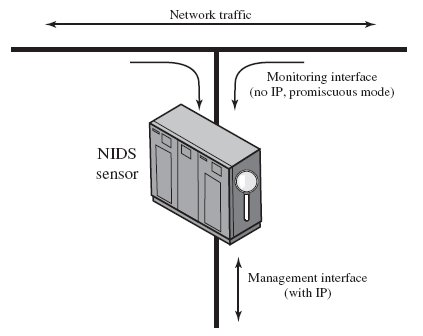
\includegraphics[width=\textwidth]{img/passive_sensor.jpg}
\caption{Illustration eines passiven NIDS Sensors} \label{fig1}
\end{figure}

\section{Eventuell Snort}


%Bibliographie
\begin{thebibliography}{8}
\bibitem{ref_article1}
Rathore, Neeraj: Ethical Hacking \& Security against Cyber Crime. i.-manager's Journal on Information Technology \textbf{5}(1), 13--17 (2015-2016)

\bibitem{ref_url1}
Forbes, \url{https://www.forbes.com/sites/daveywinder/2020/01/29/google-confirms-it-will-pay-android-pixel-hackers-15-million/?sh=2dbb025833ab}. Last accessed 15 Dec 2021

\bibitem{ref_url2}
techjury, \url{https://techjury.net/blog/how-many-cyber-attacks-per-day/}. Last accessed 15 Dec 2021

\bibitem{ref_url3}
University of Maryland, \url{https://eng.umd.edu/news/story/study-hackers-attack-every-39-seconds}. Last accessed 15 Dec 2021

\bibitem{ref_url4}
Wired, \url{www.wired.com/story/worst-hacks-of-the-decade}. Last accessed 15 Dec 2021

\bibitem{haystack_ids}
I. Kandrouch, N. Hmina, H. Chaoui
:A Novel Security Architecture Based on 
Haystack System for HDFS Storage System: 
Extended Work, S. 714, (2020)

\bibitem{IDS_Book_1}
Roberto Di Pietro, Luigi V. Mancini: Intrusion Detection Systems, S. 173, (2008)

\bibitem{IDS_Book_2}
William Stalling, Lorie Brown: Computer Security Principles and Practices, 4th Edition, S. 278 - 306, (2018) 

\bibitem{url_sensors}
Wired, \url{https://www.informit.com/articles/article.aspx?p=782118}. Letzter Zugriff: 23. Dec 2021

\bibitem{ref_book_attack_1}
Martin Kappes: Netzwerk- und Datensicherheit, S. 141-142, 2nd edn Springer Vieweg (2013)
\bibitem{ref_book_attack_2}
Martin Kappes: Netzwerk- und Datensicherheit, S. 249, 2nd edn Springer Vieweg (2013)
\bibitem{ref_book_attack_3}
Martin Kappes: Netzwerk- und Datensicherheit, S. 250-251, 2nd edn Springer Vieweg (2013)

\bibitem{ref_book_attack_4}
Steffen Wendzel: IT-Sicherheit für TCP/IP- und IoT-Netzwerke, 1st edn Springer Vieweg S. 212-213 (2018)
\bibitem{ref_book_attack_5}
Steffen Wendzel: IT-Sicherheit für TCP/IP- und IoT-Netzwerke, 1st edn Springer Vieweg S. 213-214 (2018)
\bibitem{ref_book_attack_6}
Steffen Wendzel: IT-Sicherheit für TCP/IP- und IoT-Netzwerke, 1st edn Springer Vieweg S. 233 (2018)

\bibitem{ref_book_attack_7}
Claudia Eckert: IT-Sciherheit, 10th edn De Gruyter Oldenburg S. 75-76 (2018)

\bibitem{ref_url5}
Virtual Box Homepage, \url{https://www.virtualbox.org/wiki/Virtualization} \url{https://www.virtualbox.org/}. Letzter Zugriff: 45. Dec 2021

\bibitem{ref_url6}
Kali Homepage, \url{https://www.kali.org/features/}. Letzter Zugriff: 14. Dec 2021

\bibitem{ref_url7}
Nmap Homepage, \url{https://nmap.org/man/de/index.html}. Letzter Zugriff: 14. Dec 2021

\bibitem{ref_url8}
Wireshark Homepage, \url{https://www.wireshark.org}. Letzter Zugriff: 14. Dec 2021

\bibitem{ref_url9}
Cloudflare Learning, \url{ https://www.cloudflare.com/de-de/learning/ddos/ddos-attack-tools/how-to-ddos/}. Letzter Zugriff: 15 Dec 2021

\bibitem{ref_url10}
Geekflare Homepage, \url{https://geekflare.com/de/mitm-attack-tools/}. Letzter Zugriff: 15 Dec 2021 Letzter Zugriff: 15 Dec 2021

\bibitem{ref_ieee_attack_8}
Mauro Conti, Nicola Dragoni, Viktor Lesyk: A Survey of Man In The Middle Attacks \url{https://ieeexplore.ieee.org/abstract/document/7442758}. Letzter Zugriff: 25 Dec 2021

\bibitem{ref_url11}
Ionos Homepage, \url{https://www.ionos.de/digitalguide/server/sicherheit/man-in-the-middle-attack-angriffsmuster-im-ueberblick/} Letzter Zugriff: 25 Dec 2021

\bibitem{ref_url12}
Ionos Homepage, \url{https://www.ionos.de/digitalguide/server/sicherheit/dns-spoofing/} Letzter Zugriff: 25 Dec 2021

\bibitem{snort_book_1}
Caswell B., Baker A., Beale J.: Snort Intrusion Detection and Prevention Toolkit,
(2007)

\bibitem{snort_url}
Snort Homepage, \url{https://www.snort.org/} Letzter Zugriff: 27 Dec 2021

\bibitem{hids_url_1}
Heimdal Security Homepage, \url{https://heimdalsecurity.com/blog/host-intrusion-detection-system-hids/} Letzter Zugriff: 27 Dec 2021

\bibitem{hids_url_2}
Redscan Homepage, \url{https://www.redscan.com/services/managed-intrusion-detection-system/hids/} Letzter Zugriff: 27 Dec 2021


% http://infosecwriters.com/text_resources/pdf/Footprinting.pdf



%\bibitem{ref_lncs1}
%Author, F., Author, S.: Title of a proceedings paper. In: Editor,
%F., Editor, S. (eds.) CONFERENCE 2016, LNCS, vol. 9999, pp. 1--13.
%Springer, Heidelberg (2016). \doi{10.10007/1234567890}

%\bibitem{ref_book1}
%Author, F., Author, S., Author, T.: Book title. 2nd edn. Publisher,
%Location (1999)

%\bibitem{ref_proc1}
%Author, A.-B.: Contribution title. In: 9th International Proceedings
%on Proceedings, pp. 1--2. Publisher, Location (2010)

%\bibitem{ref_url2}
%LNCS Homepage, \url{http://www.springer.com/lncs}. Last accessed 4
%Oct 2017
\end{thebibliography}
\end{document}
